\documentclass[a4paper]{book}

% Load the VUB package.
% This has many options, please read the documentation at
% https://gitlab.com/rubdos/texlive-vub
\usepackage{vub}

\usepackage{graphicx}
\graphicspath{ {./images/} }


% Some highly suggested packages, please read their manuals.
%\usepackage{cleveref}
\usepackage[natbib,style=apa]{biblatex}
\addbibresource{references.bib}

\title{Distributing first-class reactors in a cluster environment}
\pretitle{\flushleft{Graduation thesis submitted in partial fulfilment of the requirements for the degree of de Ingenieurswetenschappen: Applied informatics}}
%\subtitle{Haai Virtual machine}
\author{Hans Van der Ougstraete}
\date{June~2024}
\promotors{Promotors: prof.\ dr.\ Wolfgang De Meuter,\and prof.\ dr.\ Joeri De Koster \and Supervisor: Bjarno Oeyen}

\faculty{sciences and bioengineering sciences} % Note: without the word "Faculty"!

\begin{document}
\frontmatter
\maketitle%

% Oftentimes, you need add a second language title.
\title{Distributing first-class reactors in a cluster environment}
\pretitle{\flushleft{Proefschrift ingediend met het oog op het behalen van de graad van Master of Science in de Ingenieurswetenschappen: Toegepaste informatica}}%
%\subtitle{mijn ondertitel}
\date{Juni~2024}%
\promotors{Promotors: prof.\ dr.\ Wolfgang De Meuter, \and prof.\ dr.\ Joeri De Koster \and Supervisor: Bjarno Oeyen}
\faculty{wetenschappen en bio-ingenieurswetenschappen}%
\maketitle%

\chapter{Abstract}
This thesis delves into the realm of distributed reactive programming, focusing on the distribution model for the purely reactive language Haai. Utilizing the actor model, the Haai language is distributed across a cluster of Elixir nodes, leveraging a shared-nothing approach to facilitate scalability and deployment. A validation of this distribution model is performed through an experiment involving a distributed reactive melody generator, which reacts to incoming streams of numbers by computing consonant frequencies and sound durations. This thesis addresses the challenge of distributed reactive programs, a task made complex by delays, network failures, and other distributed system issues. By exploring distribution models for reactive programming languages, this research contributes to understanding the intricacies of reactive systems in distributed settings.

Keywords: Reactive programming, Distribution, Haai, Elixir, Actor model, Distributed systems.


\tableofcontents%

\mainmatter%
\chapter{Introduction}

Reactive programming has been around for a while, gaining traction in various domains due to its ability to handle asynchronous and event-driven scenarios effectively. One of its notable advantages lies in its suitability for distributed systems. By its nature, reactive programming facilitates the development of systems that can easily scale across distributed environments, allowing components to communicate asynchronously and react to events in real-time. However, distributing reactive programming poses several challenges (\cite{DBLP:journals/csur/BainomugishaCCMM13}) such as consistency, coordination, fault tolerance and many more. These challenges highlight the need for further research and study in understanding how reactive programming principles can be effectively applied and scaled in distributed environments. By investigating these challenges, we can gain insights into best practices and architectural approaches for building robust and scalable distributed reactive systems.

\section{Reactive programming}
Reactive Programming is a broader programming paradigm that encompasses the idea of reacting to changes and events in a system. It involves modeling the flow of data as streams of events and using declarative and composable abstractions to handle asynchronous and event-driven scenarios. Reactive Programming emphasizes building systems that are responsive, scalable, and resilient by design.

Let's consider a simple example to illustrate reactive programming: Imagine you're building a weather application that displays real-time temperature updates for a city. In a reactive programming approach, whenever there's a new temperature reading from the weather API, it gets emitted as an event in the rp program.

Now, let's say you have various components in your application that need to react to these temperature updates. For instance, you have a component that displays the current temperature, another component that triggers an alert when the temperature goes above a certain threshold, and yet another component that logs the temperature data to a file.

With reactive programming, you can easily connect these components to the temperature data stream. Whenever a new temperature reading is emitted, all dependent components are automatically notified and can react accordingly. This ensures that your application stays in sync with the latest data without you having to manually manage the flow of information between components.

\section{Statement of the problem}
The distribution of reactive programming (RP) introduces a myriad of complexities and challenges that hinder the seamless scalability and robustness of distributed systems. While RP has demonstrated efficacy in handling asynchronous and event-driven scenarios within localized contexts, extending its principles to distributed environments poses significant hurdles. Existing problems such as consistency maintenance, fault tolerance, communication overhead, scalability bottlenecks, and data consistency issues undermine the effectiveness of distributed RP solutions. We want to gather a thorough understanding and targeted investigation into these challenges.

%\section{Overview}
The Structure of this thesis starts with an overview of related subjects in chapter 2. After which we introduce techniques and tools selected to perform the research. to end with the evaluation of the selected techniques and tools.

\chapter{Reactive programming}

Reactive programming (RP) offers a paradigm that well fit the needs for building responsive, scalable and resilient software systems. RP offers a declarative approach for handling asynchronous streams of data. A reactive program will automatically react to changes over time. We can build (soft) real time applications that react given incoming data. We could say that the program has been programmed in a declarative way to know what to do when an input is presented to the ever running reactive program. 

\section{State of the art}
RP has its roots in functional programming and event-driven architectures. Over the years, it has evolved from simple event handling mechanisms to sophisticated reactive systems that emphasize declarative and composable data flows. The advent of reactive extensions (Rx) in various programming languages, such as RxJava, RxJS, and Rx.NET, played a pivotal role in popularizing RP and standardizing its concepts across different platforms.

All of the mentioned frameworks and libraries have the downside of being composed of two components. The reactive system is build on top of an imperative language. This makes them prone to the \textit{Reactive Thread Hijacking Problem} and the \textit{Reactive/Imperative Impedance Mismatch} problems (\cite{vonder_tackling_2020}).

\section{Distributed reactive programming}

When distributing a reactive program, issues related to distributed systems come apparent in the distributed reactive program (drp). Resolving those issues becomes part of the distributed reactive program and the distributed system architecture. In this thesis we focus on the following challenges.
\begin{description}
	\item[Consistency and Coordination:] In distributed environments, maintaining consistency across different nodes can be challenging. Reactive programming relies on the propagation of changes and events, and ensuring that all nodes in a distributed system are in sync requires careful coordination and management of data flows. Different nodes may receive events in different orders, leading to potential inconsistencies that need to be addressed through synchronization mechanisms and event ordering techniques. 
	\item[Fault Tolerance and Resilience:] Distributed systems are prone to failures, whether due to network partitions, node crashes, or other issues. Reactive programming emphasizes responsiveness and fault tolerance, but distributing these principles across a network introduces new challenges in handling failures gracefully and ensuring system resilience.
	\item[Network Communication Overhead:] Asynchronous communication between distributed components in a reactive system can introduce overhead in terms of network latency and message passing. Efficiently managing this communication overhead while maintaining responsiveness is crucial for the performance of distributed reactive systems.
	
\end{description}

In the literature inconsistencies in the data are called glitches. A glitch is a momentary inconsistency in a time-varying value. For example in a financial application we do not want to read inconsistent values. We want to read the new value after the update on the values this new value depends on has been finished. Being free of glitches is called glitch-freedom. According to Margara and Salvaneschi (\cite{DBLP:journals/tse/MargaraS18}) there are two types of glitch-freedom. A 'single-source' and 'complete' way for the program to be free of glitches. In the single-source case we assume one node, all pending updates to that node are performed before the updated values is available. Complete glitch freedom is considered when we have more then one node. To have complete glitch freedom we must make sure that updates occurred in the same order for all nodes considered by this update. 

\chapter{Strategy and Methodology}

Our approach in this work is to remove as many of the issues known to rp and drp by developing a system that by design solves the challenges known to drp. The distributed system is build as a shared nothing architecture (sna) and hosts an Erlang cluster. We have chosen this architecture for basic simplicity as it allows to easily scale and monitor fault tolerance since each node is independent and self-sufficient.

To deploy the system we make use of code mobility, allowing us to declaratively define which rp needs to run on what node or group of nodes. We have build a runtime for the purely functional reactive language Haai on top of the sna. Each node represents a runtime towards which a (master) node can send the code to be deployed.

All the different nodes or runtimes in the cluster have a rhythmical organization (eg: the loop time of a reactor is a fixed value in milliseconds). The 'tempo' of each runtime will allow us to monitor the cluster for failures of nodes in the sna.  

\chapter{Purely reactive programming language}
\section{Reactors}
In Haai, a purely reactive computer language, the only construct available for expressing computations is a reactor. A reactor is a sort of blue print that will be used to deploy any number of deployments based on that reactor. We can write a single reactor or combine multiple reactors in one 'main' reactor or program. The main program is build out of reactors, these can be native or user defined. Every computation in a reactor is done by a reactor, some are native to the runtime others are user defined. For example the runtime could provide native reactors for basic arithmetic. \ref{fig:reactor} show the concept of a reactor.

\begin{figure}[h]
	\caption{Graphical representation of a reactor}
	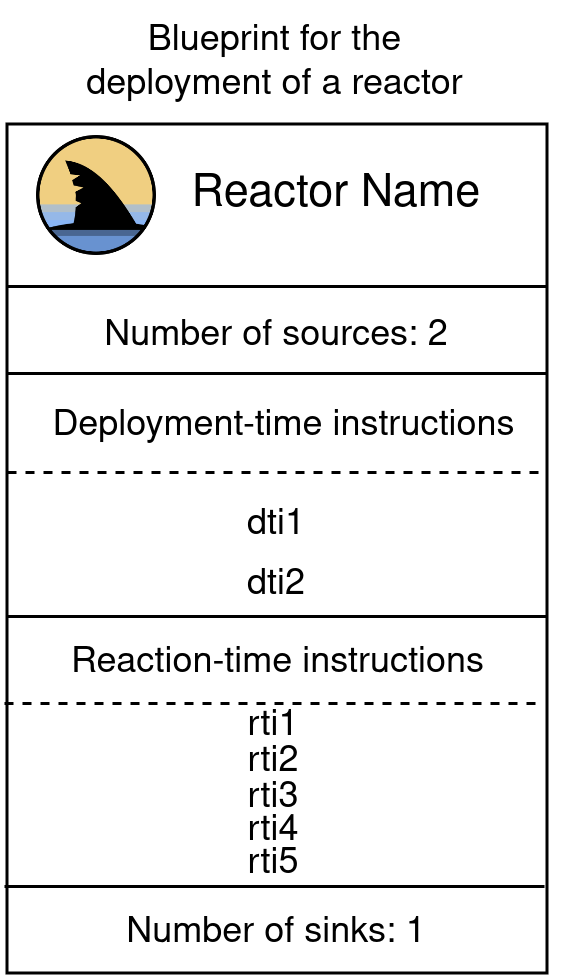
\includegraphics[scale=0.2]{reactor300.drawio}
	\centering
	\label{fig:reactor}
\end{figure}

The deployment of a reactor reacts on a data stream, that data altered by the reaction is found in the sink of the reactor. The deployment of a rector is explained in the next chapter.

\section{Haai}
We are making use of the novel purely reactive language Haai. Haai is reactive all-the-way-trough. As such the only construct available for expressing computations is a reactor. A reactor has sources or inputs and sinks or outputs. For each time the sources are updated the reactor will react and produce a new sink value. The number of sources and sinks are variable per reactor definition. In Haai there are no functions, only reactors. This allows us to build reactive programs without functions (\cite{oeyen_reactive_2024}). Different from other rp is that Haai exists out of only one layer. By design Haai solves the Reactive thread hijacking problem and the reactive/imperative impedance mismatch. 

\subsection*{Levels of reactivity}
There is a trade off where more strict levels of reactivity allow for a less wide pallet of reactive programs to be expressed. For Haai the level of reactivity will be partly defined by the computational time of the native reactors. In this implementation of the Haai virtual machine we only have native reactors that have a computational complexity of O(1). This guarantees a strong level of reactivity (\cite{oeyen_reactive_2024}).

\subsection*{Code example}
This Haai code represents three user defined reactors: consonance, duration and main. The main reactor is build out of the two user defined reactors consonance and duration and makes no use of native reactors. Consonance and duration make use of multiple native reactors to perform arithmetic. The arguments to the reactor are the sources and the keyword 'out' defines the sink of the reactor.
 
\begin{verbatim}
	
	(defr (consonance f)
	  (out (* ci f)))
	
	(defr (duration bpm)
	  (def q (/ 60000 bpm))
	  (out (* lm q)))
	
	(defr (main f bpm)
	  (out (consonance f))
	  (out (note_length bpm)))
	
	
\end{verbatim}



\section{Remus instruction set}
The Remus instruction set is the set of low-level operations that the virtual machine can execute. A Haai program or Reactor will after compilation exist out of a combination of instructions. Instructions form the Remus instruction set as listed here under. The Haai virtual machine is an implementation of this instruction set in Elixir. 
\begin{description}
	\item[[I-ALLOCMONO, reactor]] Allocate memory for the given reactor.
	\item[[I-LOOKUP, signal]] Lookup the value for signal in a signal table.
	\item[[I-SUPPLY, from, destination, index]] Supply the value found in from to destination at index.
	\item[[I-REACT, memory\_location]] Apply the reaction required at memory\_location.
	\item[[I-CONSUME, memory\_location, index]] Move the value form REACT to the run-time-memory.
	\item[[I-SINK, rti\_location, sink\_index]] Remove value from run-time-memory and store in the reactor sink.
\end{description}


\section{Example bytecode program}

After parsing the bytecode that was compiled form the original Haai code with the Haai compiler into an Elixir readable format of nested lists a program could look like this. In this example we see two user defined reactors named consonance and note\_length followed by the main reactor that represents the actual program that will be deployed. 

\begin{verbatim}
	co_nl = [
	[:consonance, 1, 1,
	[
	["I-ALLOCMONO", :multiply]
	],
	[
	["I-LOOKUP", :ci],
	["I-SUPPLY",["%RREF",1],["%DREF",1],1],
	["I-SUPPLY",["%SRC",1],["%DREF",1],2],
	["I-REACT",["%DREF",1]],
	["I-CONSUME",["%DREF",1],1],
	["I-SINK",["%RREF",5],1]]
	],
	
	[:note_length, 1, 1,
	[
	["I-ALLOCMONO", :divide],["I-ALLOCMONO", :multiply]
	],
	[
	["I-SUPPLY",60000,["%DREF",1],1],
	["I-SUPPLY",["%SRC",1],["%DREF",1],2],
	["I-REACT",["%DREF",1]],
	["I-LOOKUP",:lm],
	["I-SUPPLY",["%RREF",4],["%DREF",2],1],
	["I-CONSUME",["%DREF",1],1],
	["I-SUPPLY",["%RREF",6],["%DREF",2],2],
	["I-REACT",["%DREF",2]],
	["I-CONSUME",["%DREF",2],1],
	["I-SINK",["%RREF",9],1]]
	],
	
	[:main, 2, 2,
	[
	["I-ALLOCMONO", :consonance],["I-ALLOCMONO", :note_length]
	],
	[
	["I-SUPPLY",["%SRC",1],["%DREF",1],1],
	["I-REACT",["%DREF",1]],
	["I-SUPPLY",["%SRC",2],["%DREF",2],1],
	["I-REACT",["%DREF",2]],
	["I-CONSUME",["%DREF",1],1],
	["I-SINK",["%RREF",5],1],
	["I-CONSUME",["%DREF",2],1],
	["I-SINK",["%RREF",7],2]
	]
	]
	]
\end{verbatim}

The above is an example for reactor\_bytecode that is send into the Haai virtual machine. It is a compilation of the following Haai program defining two user defined reactors (consonance and note\_length) and making use of two native reactors (:multiply (* in Haai) and :divide (/ in Haai)) and joining them together within the main reactor. The main reactor could be seen as the 'main' function in C. The starting point or the call that kicks off the programs execution.


\chapter{Haai virtual machine}
To make it possible for Haai code to work on multiple platforms a virtual machine for each required platform is necessary. After the example of Remus, "a virtual machine that has been carefully designed to be usable for running reactive programs in low-powered computing environments."(\cite{oeyen_remus_2022}) We implement in this thesis a virtual machine for Haai. The purpose of the Haai virtual machine (Hvm) is to enable the possibility of distributing Haai programs in a cluster of machines. There are multiple reasons to distribute a reactive program like: scalability, low latency and many others. Firstly the Hvm is a prototype to investigate distribution in general and to see if at all the language works well in a distributed setting. The Hvm is developed  in the Elixir computer language. The chapter on distribution arguments our choice for Elixir. The Haai bytecode as compiled for Remus will be the representation of Haai reactors in the Hvm. 

\section{Deploying a reactor}
A reactor can be seen as a blue print for its deployment, similar how an object created from a class in object-oriented programming is an instantiation of the blueprint that the class represents. The deployment of the reactor will request a certain size of memory. That total block of memory exists out of four parts: Sources, deployment time memory (dtm), reaction time memory (rtm) and the sinks. When we go from a reactor to a deployment we can find the following information in the reactor or blue print for the deployment. The number of sources and sinks, the deployment time instructions (dti) and the reaction time instructions (rti). For each source and each sink a position is reserved in the memory block we are constructing. From the deployment time instructions in the reactor we can prepare the deployment time memory (dtm). The Dtm part of the memoryblock we are constructing will reserve space for the deployment of the reactors found in the dti. 

Now we have reserved space for the sources the sinks and dtm, the last step is to reserve space for the reaction time memory (rtm). The space required for rtm is equal to the number of instructions found in the reaction time instructions. For each instruction in rti there is one block reserved in rtm. A deployed reactor uses the four memory parts: sources, dtm, rtm and sinks to react according to the reaction time instructions found in rti. Figure \ref{fig:rde} expresses the deployment of a reactor.

\begin{figure}[h]
	\caption{Reactor deployment, from blueprint to memory block}
	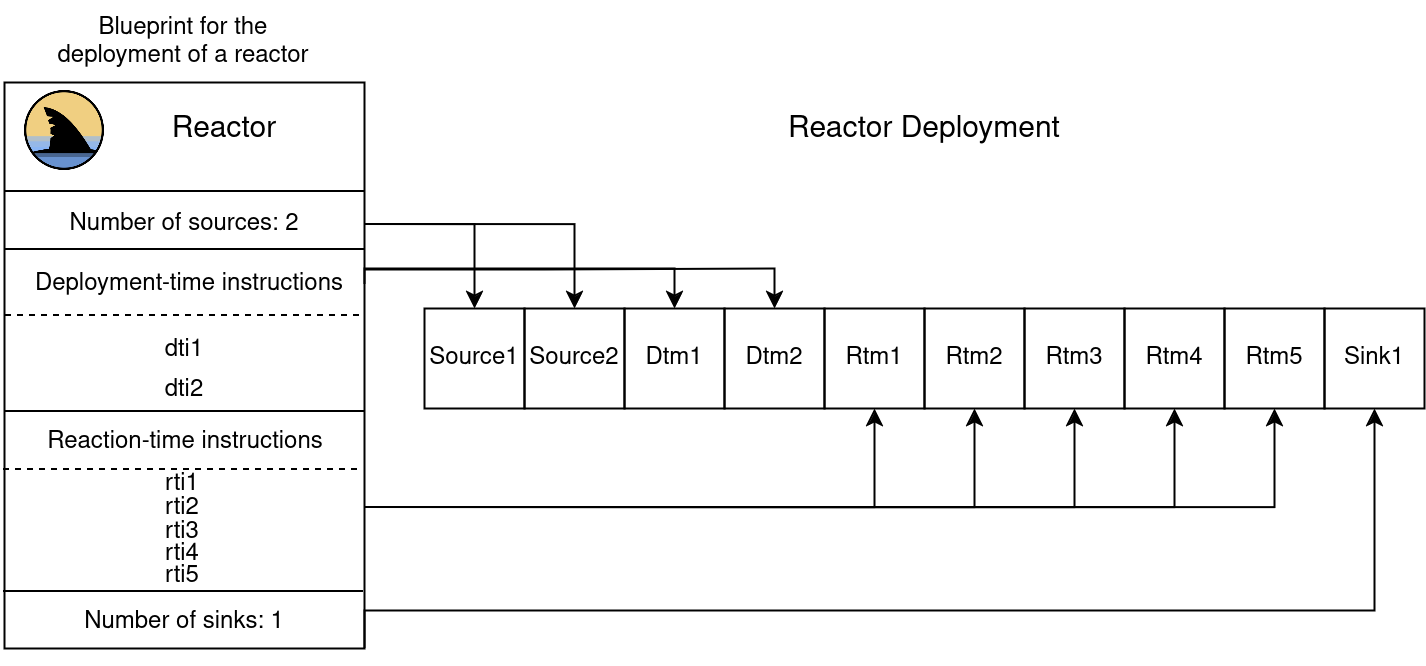
\includegraphics[width=\textwidth]{rd.drawio}
	\label{fig:rde}
\end{figure} 

\section{Running the reactor}
Running the reactor encompasses starting a Haai virtual machine with all requested arguments for the Hvm to function. The Haai virtual machine needs the following arguments to start: 
\begin{description}
	\item[Reactor bytecode] Bytecode obtained from the Haai compiler that compiles reactor definitions in the Haai language to a bytecode.
	\item[Connect source] A function that the Hvm can use to connect some input to the sources of the reactor. At each start of the next iteration this function will be called to update the sources of the deployed reactor. For example connecting to a WebSocket server to receive the data it broadcasts.
	\item[handle sink] The function that after each iteration is called to handle the new sinks produced by the deployed reactor. This function is tailored for the specific reactor that has been send as bytecode.
\end{description}

\section{Managing the reactors state}
Managing the state of a reactor is done by one actor per program or reactor deployment. The actor is build around the GenServer module in Elixir which is a behavior module that provides a generic server implementation. In this implementation the name of the GenServer is Memory. Memory is a single actor that encapsulates multiple functions to respond to various messages or calls. Together these define the behaviour of the Memory GenServer.

Memory will mainly accept calls from the runtime instructions found in the reactor deployment. Available calls are mapped on the Haai instruction set. In addition there are calls to initialize or to get or set sources and sinks into or from the Memory GenServer. One instance of Memory represents the memory block of a deployed reactor.

The GenServer module in Elixir works with calls or casts, we use calls since they are synchronous requests to the GenServer. By calling Memory in a synchronous way we make sure that the values in Memory are only accessed by one operation at a time, assuring correct values. 

\section{Native reactors}
The Haai virtual machine makes use of native reactors to perform simple arithmetic operations like addition, division, multiplication and subtraction. Native reactors are recognized by the Hvm and applied when required.

Haai is a one layer reactive programming language, contrary to two layer system where the top reactive layer can lift functions from the bottom imperative layer, Haai only uses reactors for all computation. The Hvm has a collection of frequent reactors. Thanks to the native reactors we do not need to implement the most basic reactors when composing a program. By design Haai prevents the Reactive/imperative impedance mismatch as explained in the chapter on Haai. Having the native reactors smartly covers the lack of lifting possibilities.

\chapter{Distribution}


\section{Shared-nothing architecture}
To organize the distribution of the Haai virtual machine we have opted for a shared-nothing architecture. (\cite{DBLP:journals/debu/Stonebraker86}) This allows us to build the cluster with the following characteristics, suitable for the first time distribution of the reactive language Haai.
\begin{description}
	\item[Independent Nodes] Each node can execute its own specific code and perform computations independently since no memory, storage or processing power is shared.
	\item[No shared state] Each node manages its state independently. Cluster communication between nodes is done with messages. we use Erlang distributed mechanisms in the implementation.
	\item[Horizontal scalability] Shared-nothing architectures are highly scalable horizontally, this makes it straightforward to add or remove nodes from the cluster. It allows us to run clusters of all sizes. Practically the cluster size will be bound to the available hardware.
	\item[Fault isolation] Faults or failures in one node do not affect the operation of other nodes in the system. We can monitor node failure with Erlang distributed mechanisms and act accordingly. 
	\item[Flexibility and Modularity] Changes to one node do not impact the operation of other nodes, allowing for maintenance, upgrades, and system evolution of the cluster.` 
\end{description}

\section{Erlang virtual machine}

We implemented the shared-nothing architecture in Elixir a functional, concurrent, and fault-tolerant programming language built on the Erlang Virtual Machine (BEAM). The Erlang Virtual Machine provides a robust platform due to several key features and design principles:
\begin{description}
	\item[Concurrency model] Erlang has a lightweight concurrency model which is based on actor-like processes. Since each process runs independently and can communicate with other processes trough message passing the Erlang virtual machine is inherently decentralized by design.
	\item[Fault tolerance] The BEAM VM provides mechanisms for process supervision, fault isolation, and hot code swapping, allowing systems to recover from failures without affecting the overall operation of the cluster.
	\item[Distribution transparency] Erlang's distribution features enable processes to communicate effortlessly across network boundaries. Within an Erlang cluster, nodes can seamlessly interact through remote procedure calls (RPCs) and message passing. Different types of distribution models can be build on the Erlang platform.
	\item[Scalability] Horizontal scaling or adding nodes to a cluster is straightforward. This makes it easy to scale clusters to need.
	\item[Tooling] Common tasks are simplified thanks to a comprehensive tool set. tools like the Mix build tool and the OTP framework are core tools used in the implementation of the distributed Haai cluster.
\end{description}

The example program is explained in more detail in the use case chapter. The same program or reactor can be run many times. The distributed setup we make exists out of a number of elixir nodes that all send there messages to one sound server. The bigger the distributed network is the more messages that are send to the sound server. The sound server it self has virtually no limit to receive messages. The main parts of the distribution are taken care of by the underlying Beam virtual machine. One main reason to develop the Hvm on this platform is to be able to distribute in a solid and proven way.  

\section{Actor model}
The actor system in Erlang implements the processes actor model. (\cite{de_koster_43_2016}) These actors are modeled as processes and can define there receive primitive to specify what messages it responds to. Thanks to the isolated turn principle the actor model guarantees to be free of data races and deadlocks by design.
In Erlang actors are typically used when you need to encapsulate state and behavior within a single unit of computation., actors are spawned using constructs like GenServer, Task, or Agent within a single node. All actors communicate with each other using message passing within the same node. One can use these actors for modeling concurrent and stateful components in an application.

\section{Distributed Erlang mechanisms}
Distributed Erlang mechanisms come into play when you need to communicate between actors residing on different nodes within a cluster.
Nodes communicate with each other using distributed Erlang protocols, allowing actors on different nodes to exchange messages. Distributed Erlang mechanisms provide fault tolerance, distribution transparency, and location transparency across the cluster. 

Distributed Erlang provides location transparency, allowing actors to communicate regardless of their physical location within the cluster. This transparency hides the underlying network details, promoting loose coupling (\cite{DBLP:conf/tools/CarretonMCM10}) between nodes and actors. Actors on different nodes can interact seamlessly through message passing, without needing to be aware of the specific nodes they are communicating with. Loose coupling in distributed Erlang enables the system to scale horizontally by adding or removing nodes without significantly impacting the overall architecture.

\section{Distributing the Hvm}
The Elixir cluster exist out of a number of Elixir nodes. An idle Elixir nodes is not hungry for system resources. One can easily run a ten fold of nodes on one machine to simulate a cluster. Once a number of nodes are running one of the nodes will be selected as the controller or master node. The master node will be made aware of all nodes in the cluster. With all nodes connected to the master node but not to each other we can start the deployment of reactors. Deploying a reactor on the cluster comes down to starting the Hvm on that node with the bytecode of that requested reactor. This means that all nodes can run the same or a different reactor depending on the bytecode it received. The possibility to send the actual reactor to a node, allows us to start a node to replace one that went down or to balance the number of nodes that runs a certain reactor. Code mobility works from the master node to any of the nodes in the cluster. 

Once the cluster, one master node connected to all other nodes exists, the deployment can be summarized as follows, chose a node in the cluster, a reactor bytecode, functions to connect the sources and handle the sinks and fire of. The reactor or our reactive program is started and will keep on reacting for as long as the node exist in this cluster. 

\begin{figure}[h]
	\caption{Distributing reactor deployment on Elixir cluster}
	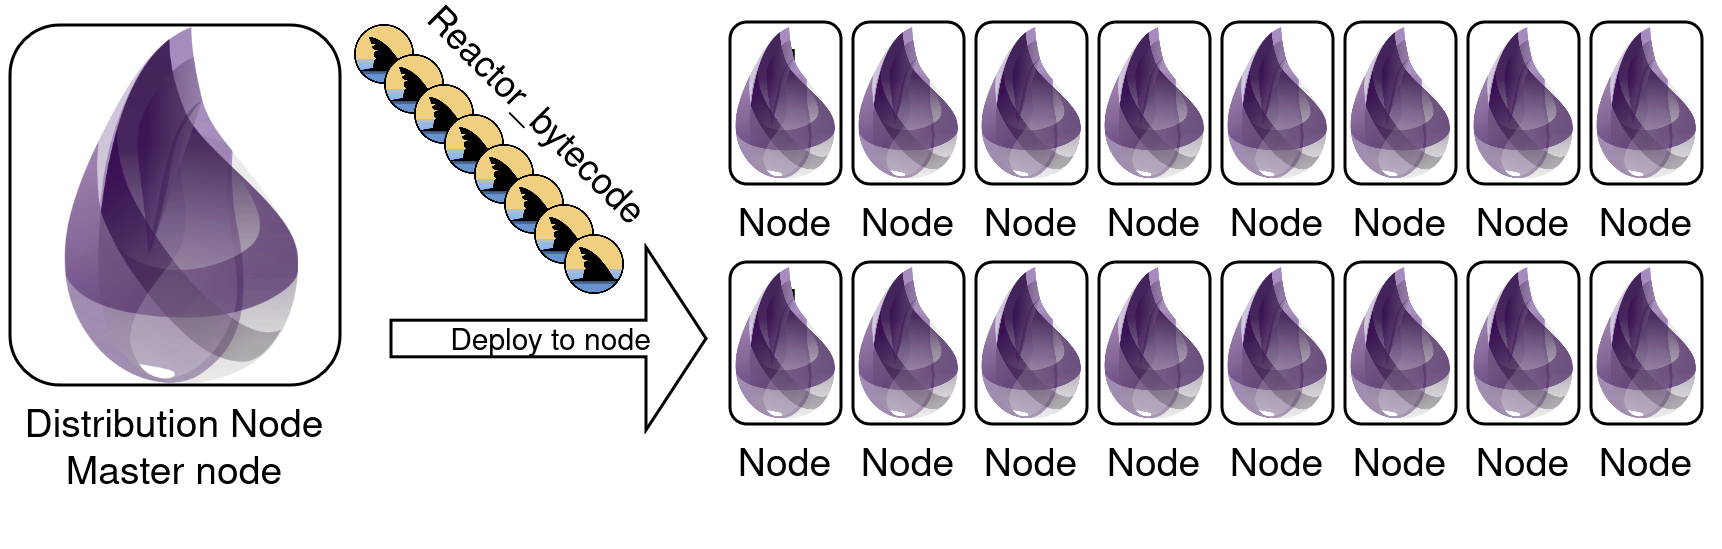
\includegraphics[width=\textwidth]{distribution300.drawio}
	\label{fig:rdi}
\end{figure}  

\chapter{Evaluation}

We monitor the rhythmical timings of the distributed reactors of the Haai reactors with sound. Each reactor is at given durations computing the next frequency to be sound on the system. This setup is very flexible as we can easily add or remove nodes from a cluster.   

\section{Distributed reactive melody generator}
The distributed Haai cluster, existing out of many distributed reactors provides the sink values form the reactors as values inserted into OSC messages (\cite{schmeder2010best}) that are send to a sound server to trigger the synthesis of some sound. It is the reactors that, by reacting on incoming streams of data, produce the values that result in a rhythmical flow of OSC messages to the sound server. 

\begin{figure}[h]
	%\caption{Diagram for the 'Distriuted Reactive Melody Generator'}
	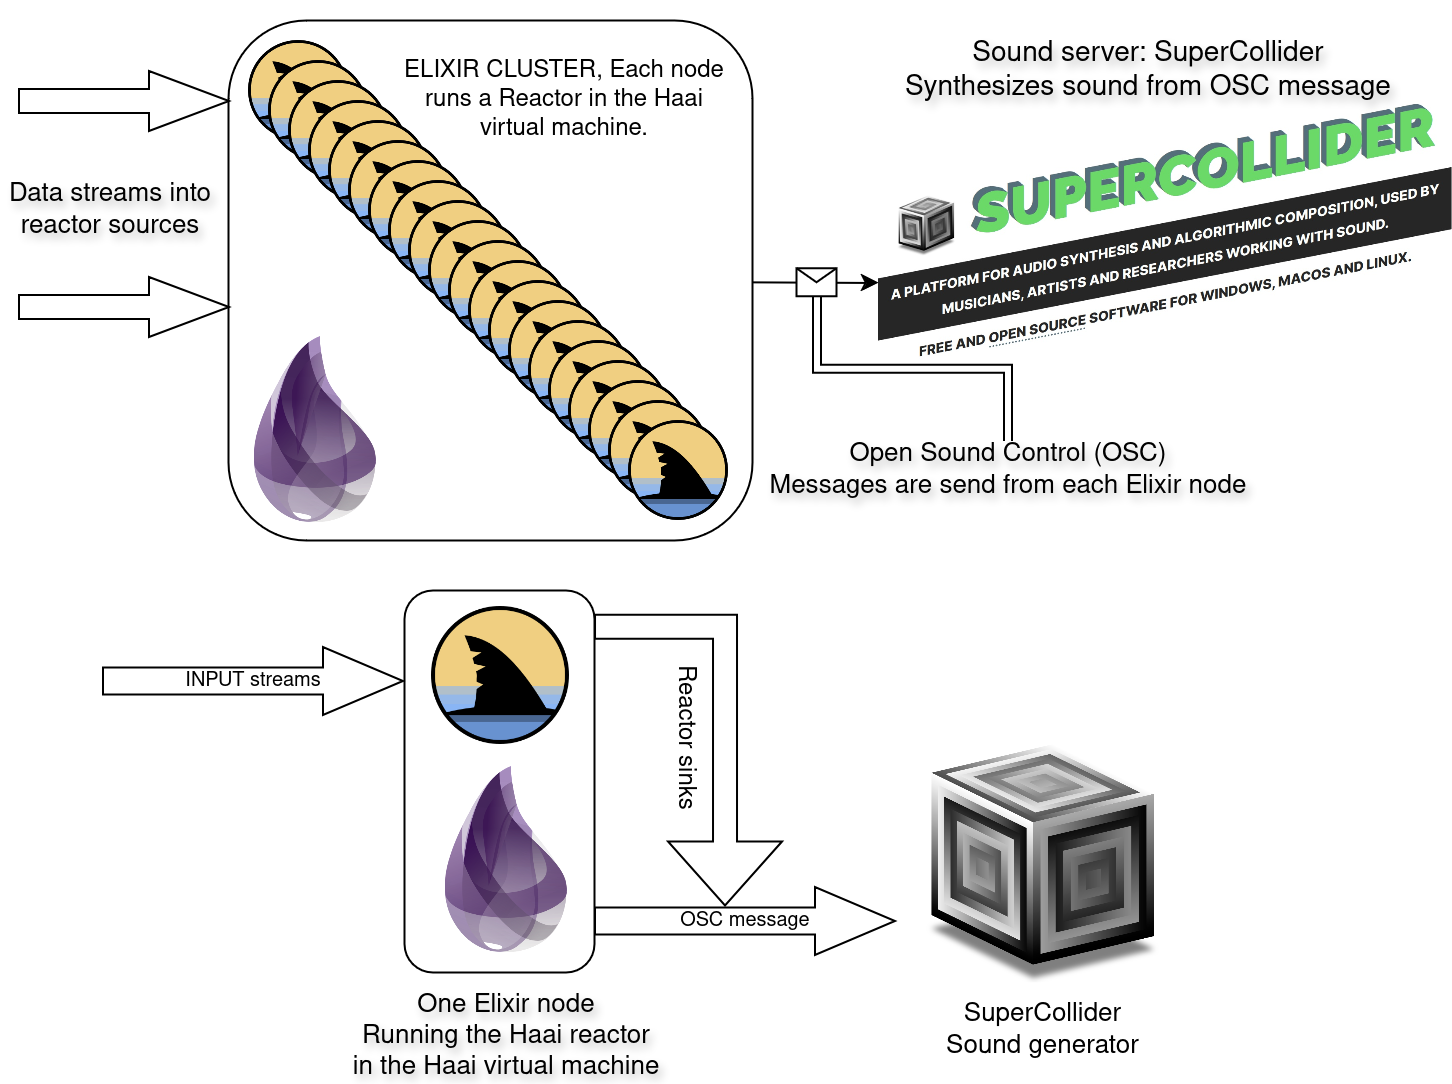
\includegraphics[width=\textwidth]{drmg200.drawio}
	\label{fig:drmg}
\end{figure}
 
The flow of rhythmical messages is related to the duration of each sound. That same duration that makes the sound disappear after it was started determines the iteration speed for the reactor or program that runs on each individual node. Each reactor iterates over and over but each iteration has a defined duration, this duration is virtually equal to the duration for a sound calculated by the reactor. A reactor will calculate the new values, sleep for the calculated duration and then provide the new values in the sink. At this point the Hvm calls a function that it was given to handle the sink values. For this use case that function constructs the message and sends it to the sound server that propagates it to the requested synthesizer. 

\section{Sound server}
The synthesizer that produces the sound is a Synthdef (the definition of a synthesizer) inside the sound server named SuperCollider. Supercollider is an open-source platform for audio synthesis and algorithmic composition. Developed by James McCartney in the late 1990s (\cite{scBook}), it has since become a powerful tool in the fields of music technology, computer music, and sound art. Supercollider provides a flexible and expressive environment for creating and manipulating sound in real-time, making it an invaluable resource for both research and artistic exploration. Some main features of super collider include:

\begin{description}
	\item[Audio Synthesis] Supercollider offers a wide range of synthesis techniques, including additive, subtractive, granular, and physical modeling synthesis. Users can create complex sounds by combining these techniques and modulating parameters in real-time.
	\item[Real-time Processing] One of Supercollider's key strengths is its ability to process audio in real-time. This makes it suitable for live performances, interactive installations, and other time-sensitive applications.
	\item[Algorithmic Composition] Supercollider provides tools for generating music algorithmically, allowing users to create compositions based on mathematical algorithms, rulesets, or generative processes.
	\item[Integration with External Hardware] Supercollider can interface with external MIDI controllers, audio interfaces, and other hardware devices, enabling users to incorporate physical instruments and sensors into their sound projects.
	\item[Community and Documentation] Supercollider has a vibrant online community of users who share code, tutorials, and resources. Additionally, comprehensive documentation is available, including tutorials, reference guides, and examples to help users learn and master the software.
	
	
\end{description}

SuperCollider has been and still is actively used in academia for many purposes, for example:
\begin{description}
	\item[Research in Music Technology] Digital signal processing, human-computer interaction, and machine learning for music. Researchers leverage its flexibility and programmability to prototype new algorithms, experiment with novel synthesis techniques, and investigate the perceptual and cognitive aspects of sound.
	\item[Composition and Sound Design] Supercollider is used to create innovative works that push the boundaries of traditional music and sound art. Its ability to generate complex and evolving textures, as well as its support for algorithmic composition, makes it a valuable tool for exploring new sonic territories.
	\item[Teaching and Learning] Supercollider is increasingly incorporated into music technology and computer music curricula at universities and colleges worldwide. It provides students with hands-on experience in sound synthesis, programming, and digital audio processing.

\end{description} 
\section{Sound server communication}
The communication between the nodes in the Elixir cluster and the sound server is done over the network using the UDP network protocol. The sound server can handle a virtual unlimited amount of messages, but is practically bounded to the udp buffer size on the actual machine that runs the sound server. As such the Elixir cluster of reactors can be of any feasible size and the sound server will respond on any number of messages by synthesizing the requested sound. 

\section{Musical values}
The reactor or program that runs on all nodes in the cluster does for each note the following. It calculates two values given two input streams of numbers. The first source is a stream of base frequencies, represented as a float number, the second source is again a stream of numbers representing a tempo in beats per minute (bpm)

\subsection*{Consonant notes}
Consonant notes sound harmonious when played together. consonance can be expressed as a ratio between two notes or frequencies. Ratios like the perfect fifth (frequency ratio of 3:2) and the major third (frequency ratio of 5:4) are very commonly used ratios in a musical setting. One of the two reactors in the main program used for this use case calculates such a note for a given base note, both are expressed in there actual frequency represented as a float number.

\subsection*{Tempo}
We can express the speed of a musical note progression in beats per minute (bpm). From that number we can then calculate the duration of individual notes in the musical performance. 

We calculate the time in milliseconds. Since one minute is 60000 milliseconds one can calculate the length of a quarter note with \(q = \frac{60000}{bpm}\) with the assumption that we use a 4/4 time signature. From the length of the quarter note it is easy to find other durations. For example, the duration of a halve note is double that of a quarter note or the duration of a eight note is half the time of a quarter note.

One of the two reactors in the main program used for this use case calculates exactly that, the length for a quarter note and improvises a deviser or multiplier to produce some duration. 

\section{Evaluating the distribution model}
The amount of messages received to monitor the nodes is one per reactor cycle. This distribution model allowed us to.............
%\backmatter
\chapter{Conclusion}
The drmg project worked well, suggesting that the actor model is a good choice to distribute Haai in a shared-nothing cluster. The number of nodes that simulate the cluster can easily be a tenfold. The reactors itself have a very light computational cost existing out of some basic arithmetic operations. One Elixir node would consumes about 90MB of memory and virtually no processor time when idle and about 3\% when performing the calculation.

\section{Further work}
Further work can be organized to explore different distribution models on the same Elixir set of nodes. Where all nodes did react independently of each other, in future work communication between nodes can be explored and more different programs or reactors can be setup and linked together...
Study glitch avoidance 

\printbibliography
\end{document}
